\chapter{Introduction} \label{ch:introduction}

\section{Concept and Motivation}
% What are we trying to get done here?
% Navigating a humanoid robot.
% Crawling a humanoid robot.
% Why are we trying to get these things done?
% Navigating is a fundamental thing for mobile robots.
% Crawling gives the robot another mode of locomotion and allows it to get to
% more places.

\begin{figure}[h!]
	\centering
	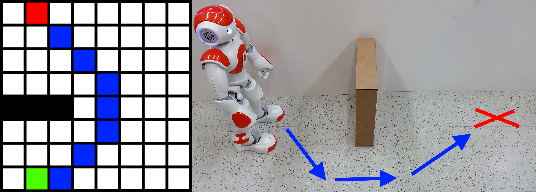
\includegraphics{nao_with_obstacle_and_map1.png}
	\caption
	{Example illustration of the Nao humanoid robot in an environment with an obstacle. The red X represents a goal
		location with the blue arrows showing an possible path. On the left side is one possible representation
		of the environment as a 2D grid.}
	\label{fig:nao_with_map1}
\end{figure}

\section{Background}
% Review previous work here as well.
% What is the problem of navigating, briefly.
% What is the problem of crawling, briefly.
% Why humanoids?
% Who's done humanoids before?
% Who's done navigation?
% We've done navigation.
% Who's done crawling?
% - Approaches to solving the problem - CPG actor critic paper
% We've done crawling.

\section{Platform Overview}

\begin{figure}
	\centering
	\includegraphics[width=0.4\textwidth]{nao_coronal_highlighted2.png}
	\caption
	{Coronal view of the Nao humanoid with a few pertinent features highlighted. }
	\label{fig:nao_diagram1}
\end{figure}

% What equipment did we use?
% - Nao
% - Lidar
% - Mount
% Why did we use these things?

\section{Navigation}
% Briefly, what's navigation?
% What approach did we go for?
% Why did we go for this?

\section{Crawl Gait}
% Briefly, what's crawling?
% Why crawling?
% What approach did we go for?
% Why did we go for this approach?

\section{Thesis Structure}
This thesis is organized as follows: 

% Chapter \ref{ch:platform} reviews the Nao Humanoid Platform with Hokoyu Scanning Laser Rangefinder augmentation.
% The navigation system is broken into three parts, 
% Chapter \ref{ch:navigation} discusses the GODZILA algorithm used for local navigation.
% Chapter \ref{ch:crawl_gait} discusses the Projected Profile crawling gait used to perform the crawl.
% Simulations and experimental results are shown in Chapters \ref{ch:simulations} and \ref{ch:results}, 
% while a discussion of the work is given in Chapter \ref{ch:conclusion}.
